\documentclass[10pt,twocolumn,letterpaper]{article}

\usepackage{cvpr}
\usepackage{times}
\usepackage{epsfig}
\usepackage{graphicx}
\usepackage{amsmath}
\usepackage{amssymb}

% Include other packages here, before hyperref.

% If you comment hyperref and then uncomment it, you should delete
% egpaper.aux before re-running latex.  (Or just hit 'q' on the first latex
% run, let it finish, and you should be clear).
\usepackage[pagebackref=true,breaklinks=true,letterpaper=true,colorlinks,bookmarks=false]{hyperref}


\cvprfinalcopy % *** Uncomment this line for the final submission

\def\cvprPaperID{****} % *** Enter the CVPR Paper ID here
\def\httilde{\mbox{\tt\raisebox{-.5ex}{\symbol{126}}}}

% Pages are numbered in submission mode, and unnumbered in camera-ready
\ifcvprfinal\pagestyle{empty}\fi
\begin{document}

%%%%%%%%% TITLE
\title{A Comparison of Different Face Recognition Algorithms}

\author{\begin{tabular}{l c r}Yi-Shin Liu & Wai-Seng Ng & Chun-Wei Liu \end{tabular} \\
National Taiwan University\\
{\tt\small \{sitrke,markng,dreamway\}@cmlab.csie.ntu.edu.tw}
% For a paper whose authors are all at the same institution,
% omit the following lines up until the closing ``}''.
% Additional authors and addresses can be added with ``\and'',
% just like the second author.
% To save space, use either the email address or home page, not both
}

\maketitle
\thispagestyle{empty}

%%%%%%%%% ABSTRACT
\begin{abstract}
    We make a comparison of five different face recognition algorithms.
    Four existed algorithm and a new Ensemble Voting Algorithm were be
    implemented. The algorithms training on a data set with 1815 faces,
    registering on a gallery set with 1027 faces,
    and test on four different probe sets. This paper will detail
    the parameter tuning process, and report the testing result via 
    receiver operating characteristic (ROC) curve and verification accuracy.
\end{abstract}

%%%%%%%%% BODY TEXT
\section{Introduction}

Face Recognition has been researched for several years, different type of
methods tried to solve two major problems in this area: face identification
, and face verification. Face identification try to indicate the identity
of a visitor. Fisherfaces~\cite{Belhumeur1997} and Local Binary Patterns 
(LBP)~\cite{Ahonen2004} perform well in this function; In the other hands, face
verification, which try to verify if a visitor is truly as his claim. Facial Trait
Code (FTC)~\cite{Lee2008} and the Ensemble Voting Algorithm (EVA) perform well. The Eigenfaces
~\cite{Turk1991} will be mention as a reference. We briefly introduce these methods below.

\subsection{Related Works}
Principle component analysis (PCA) is widely used for dimensionality reduction,
Turk and Pentland introduce Eigenfaces in 1991~\cite{Turk1991}. By this method, 
the dimensionality of a face model can be reduced from image pixel size to several 
principle basis, the basis may encode sufficient information about the face.
However, it is designed in a way to best preserve data in the embedding space,
and consequently cannot promise good discriminating capability.

Linear discriminant analysis (LDA) is also used for dimensionality reduction,
and it provide a good discriminating capability. Fisherfaces~\cite{Belhumeur1997}
improve the face recognition system, but the drawback of this method is it
can not perform well in face verification.

LBP is a powerful method to solve face recognition problem, it is efficient and
also easy to implement. The drawback is it is hard to determine a verification
threshold, which mean the boundary between imposter and guest is hard to 
determine in chi square distance matrix space.

FTC has good performance on verification, its distance matrix in discrete integer
space helping us tuning verification easier than other methods. In contrast to
setting the threshold, tuning the parameters of FTC are really complicated and 
time-consuming, we do lots of efforts on this algorithm.
Thus, tuning FTC is the bottle neck of the project.

\subsection{Our Approach}
Ensemble Voting Algorithm (EVA) tries to gather different opinions of face recognition
algorithms, and votes for a common idea for final decision. The algorithm 
achieve $95\%$ accuracy in a random sample $20$ faces set contained imposter and gallery face.

We will introduce the methods, and detail the parameter tuning process of 
five algorithms in section 2., most of content will focus on FTC's tuning. 
And then we discuss the performance on different algorithms, 
the ROC curve and highest precision will be reported in section 3.. 
In the end of the paper, we will discuss the whole system and make a conclusion.

%-------------------------------------------------------------------------

\section{Implementation and Tuning}
We describe the implementation and parameter tuning process in this section.
Each section will briefly explain the approach of implementation, and show
a figure illustrated the relation ship between accuracy and different types
of parameters. We decide the parameter
for testing is based on overall performance in different data sets.

\subsection{Eigenfaces}
Eigenfaces was proposed by Turk and Pentland in 1991~\cite{Turk1991}. The idea takes a face
as a column vector of pixels $x$, where the length of the vector $d$ represents
the product of patch's width and height.
Suppose we have $n's$ faces $x_1, x_2, ..., x_n$,
denote the faces as a matrix $X=\{x_1, x_2, ..., x_n\}$.
We training the Eigenfaces model of these data in the following steps:
\begin{center}
    \begin{enumerate}
        \item Compute the scatter matrix $S=(X-M)(X-M)^T$, where $M$ is a matrix
              that each column represents the mean vector $\mu$ of $x_1, x_2, ..., x_n$.
        \item Solve the eigenvalues of $S$, pick the eigenvectors of $k's$ 
              largest eigenvalue as the basis of $X$.
    \end{enumerate}
\end{center}
The output model is a matrix $E$ which concatenates $k's$ eigenvectors.
The model is used to linearly project an input vector $x$ as $y=E^Tx$.

Clearly, the tuning factors are $k$, the dimensionality of projected vector $y$; and
also the input image pixels $d$.
We plot the dimensionality-accuracy curve in Figure~\ref{fig:pca_par}
to see the performance.

\begin{figure}[t]
    \begin{center}
        %\fbox{\rule{0pt}{2in} \rule{0.9\linewidth}{0pt}}
        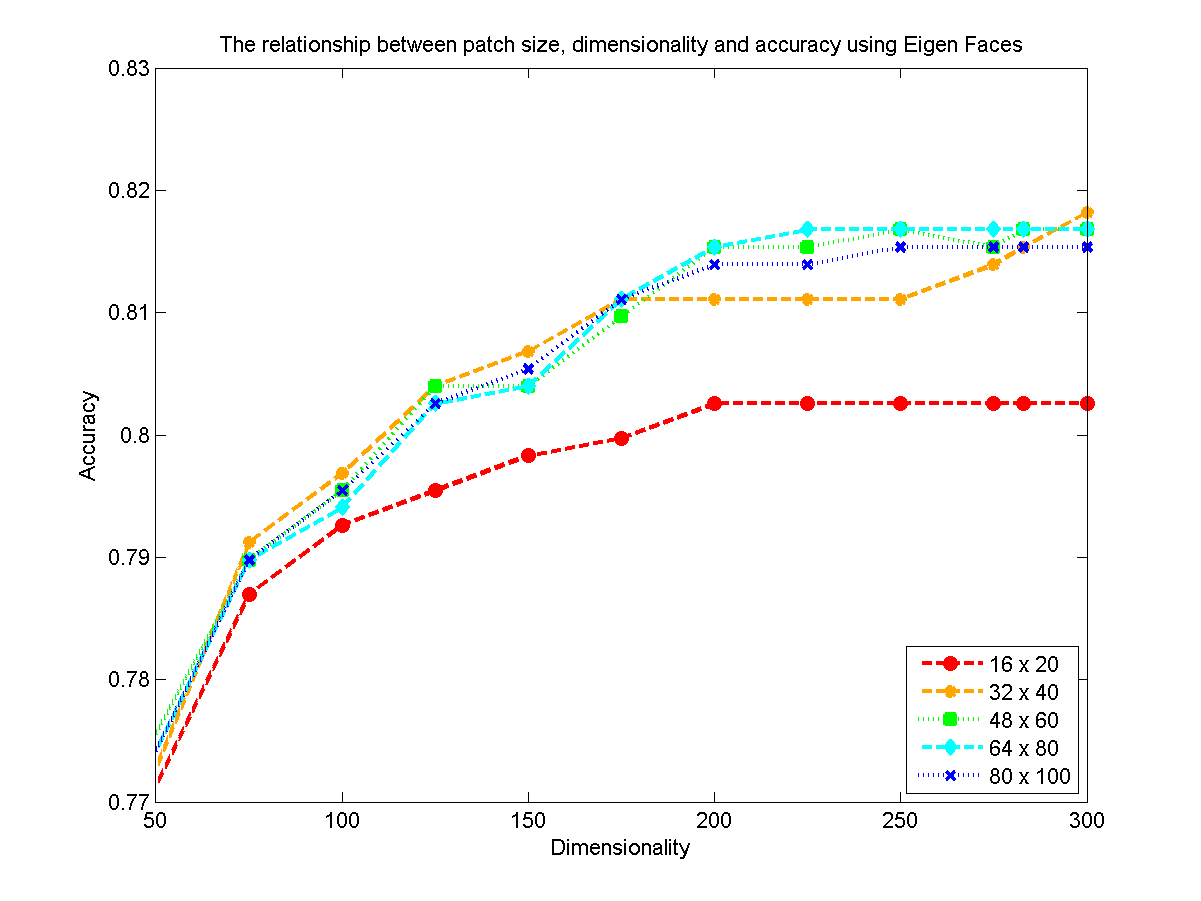
\includegraphics[width=0.8\linewidth]{fig/pca/pca_par.png}
    \end{center}
    \caption{Accuracy of PCA in different parameters.}
    \label{fig:pca_par}
\end{figure}

As our respect, too large patches are not useful in PCA case. Because we only have 1815
faces, but the data would separated in 8000 dimensionalities if we used $80*100$ patch size.
Therefore a curse of dimensionality effect is be respected. The accuracy of PCA will 
be limited by increasing the dimensionality after projected, because the last eigenvector
is not as importance as first one. 

We weighted average the accuracy of different probe sets. They are $294$ images in the neutral
, $111$ in the illumination, $246$ in the expression, and $53$ in the pose faces data set.
The best average performance in the pose sets is achieved by $d=64*80$ and $k=300$, we choose them for testing.

%-------------------------------------------------------------------------

\subsection{Fisherfaces}
Fisherfaces was proposed by Belhumeur \etal in 1997~\cite{Belhumeur1997}. 
The idea is same as Eigenfaces, but using discriminable linear projection model. 
Therefore, the scatter matrix is divided into the between-class scatter matrix
which be defined as
\[
    S_B=\sum^c_{i=1}N_i(\mu_i-\mu)(\mu_i-\mu)^T
\]
and the within-class scatter matrix which be defined as
\[
    S_W=\sum^c_{i=1}\sum_{x_k\in X_i}(x_k-\mu_i)(x_k-\mu_i)^T
\]
where $\mu_i$ is the mean image of class $X_i$, and $N_i$ is the number of samples
in class $X_i$, total $c$ classes. The model of Fisherfaces is trained as the following steps:
\begin{center}
    \begin{enumerate}
        \item Training the PCA model for $X$, and linearly project $X$ into $k's$ dimensionality $Y$.
        \item Compute the scatter matrices $S_B$ and $S_W$ of $Y$.
        \item Solving the eigenvalues of ${S_W}^{-1}S_B$, pick all eigenvectors as the basis of $X$.
    \end{enumerate}
\end{center}
Same as before, a linear projection model is established. The model is a concatenation of
$k's$ eigenvectors we solved above.

The parameters are $k$ and $d$, we plot the average accuracy of LDA in Figure~\ref{fig:lda_par}.

\begin{figure}[t]
    \begin{center}
        %\fbox{\rule{0pt}{2in} \rule{0.9\linewidth}{0pt}}
        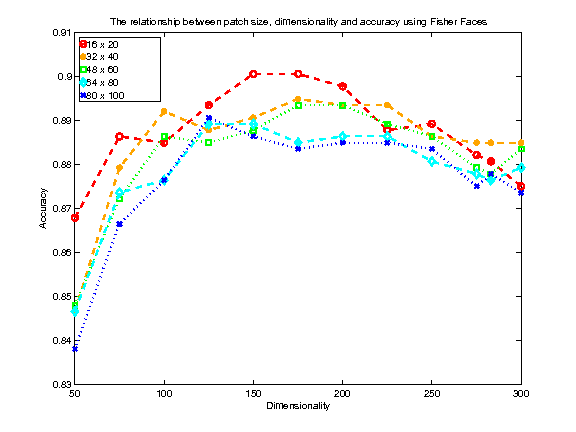
\includegraphics[width=0.8\linewidth]{fig/lda/lda_par.png}
    \end{center}
    \caption{Accuracy of LDA in different parameters.}
    \label{fig:lda_par}
\end{figure}

Too large dimensionality after projected are useless. It is because the reserve information
is not principle component. The parameters $k=150$ and $d=16*20$ is chose for testing.

%-------------------------------------------------------------------------

\subsection{Local Binary Patterns}
Local Binary Pattern used in face recognition was proposed by 
Ahonen \etal~\cite{Ahonen2004}. The method provide information about the
shape and the texture. The original LBP operator labels the pixels of an
image by thresholding the $3*3$-neighbourhood of each pixel with the center
value and consider the results as a binary number, and we make a histogram
to describe the image. Here we use the extension to original operator called
{\it uniform pattern}. A LBP is called uniform if it contains
at most two bitwise transitions from $0$ to $1$. With this criteria, 
the number of bins of different patterns reduced from $256$ to $59$,
$58$ bins for different uniform patterns, and one bin for nonuniform patterns.
A image is divided by $p*p$ patches, each of them have a histogram of LBP.
The histogram will be concatenated as a $p*p*59$ vector feature descriptor.

The parameters are the divided number $p$, and the input images pixel $d$.

\begin{figure}[t]
    \begin{center}
        %\fbox{\rule{0pt}{2in} \rule{0.9\linewidth}{0pt}}
        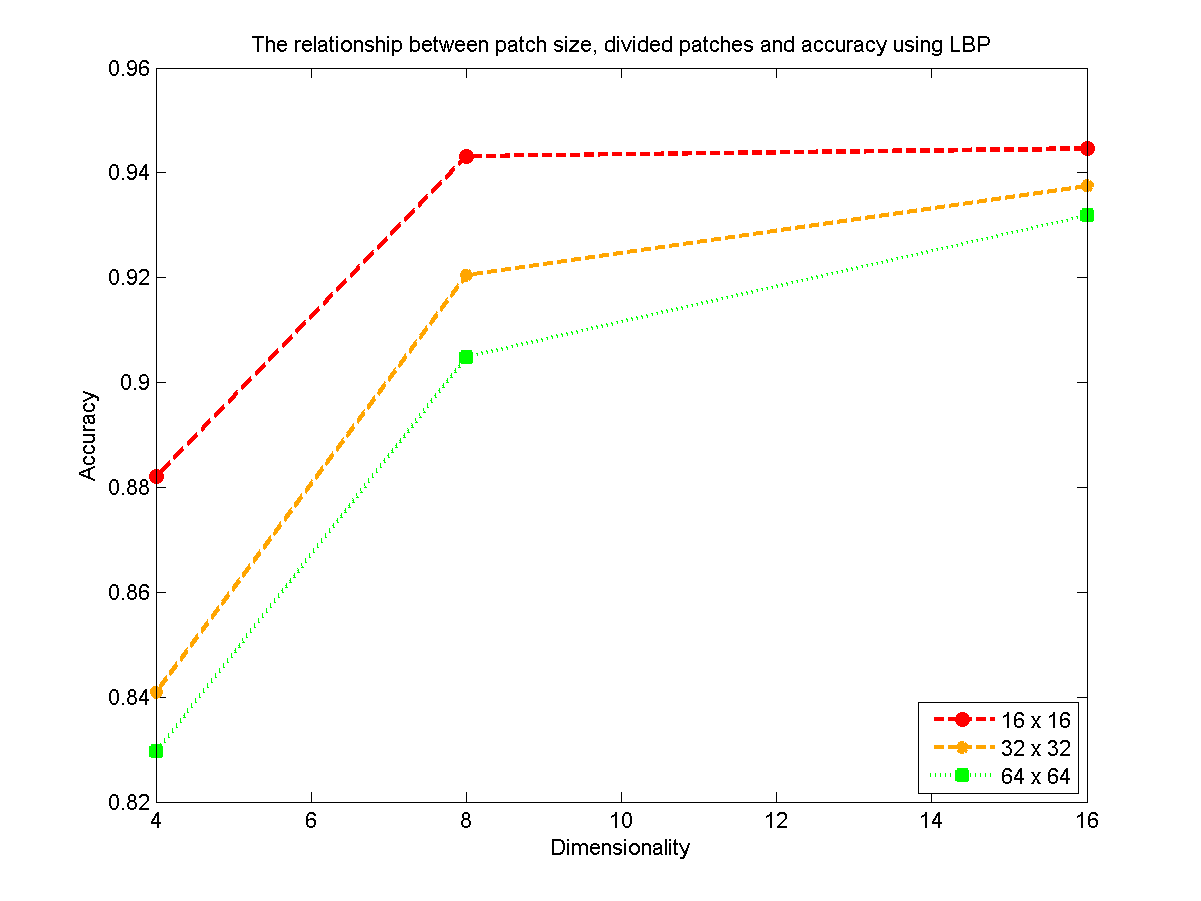
\includegraphics[width=0.8\linewidth]{fig/lbp/lbp_par.png}
    \end{center}
    \caption{Accuracy of LBP in different parameters.}
    \label{fig:lbp_par}
\end{figure}

In the experiment, we find out if $p$ is bigger, the result always be better.
The image size $64*64$ is most suitable for all cases. In the end, we decide
$d=64*64$ and $p=8$ for testing. Moreover, LBP reaches a highest accuracy, 
we will report it in Section 3..

%-------------------------------------------------------------------------

\subsection{Facial Trait Code}
Facial Trait Code is used to represent a face image, it was proposed
by Lee \etal in 2008~\cite{Lee2008}. The idea is to mark a local patch from face image
to several classes, and use different coded local patches to represent a face.
A local patch, so called facial trait, will be projected by PCA and LDA to 
reduce the dimensionality, and extract the feature for clustering. The
features which are clustered together will be seen as same class. 

\begin{figure}[t]
    \begin{center}
        %\fbox{\rule{0pt}{2in} \rule{0.9\linewidth}{0pt}}
        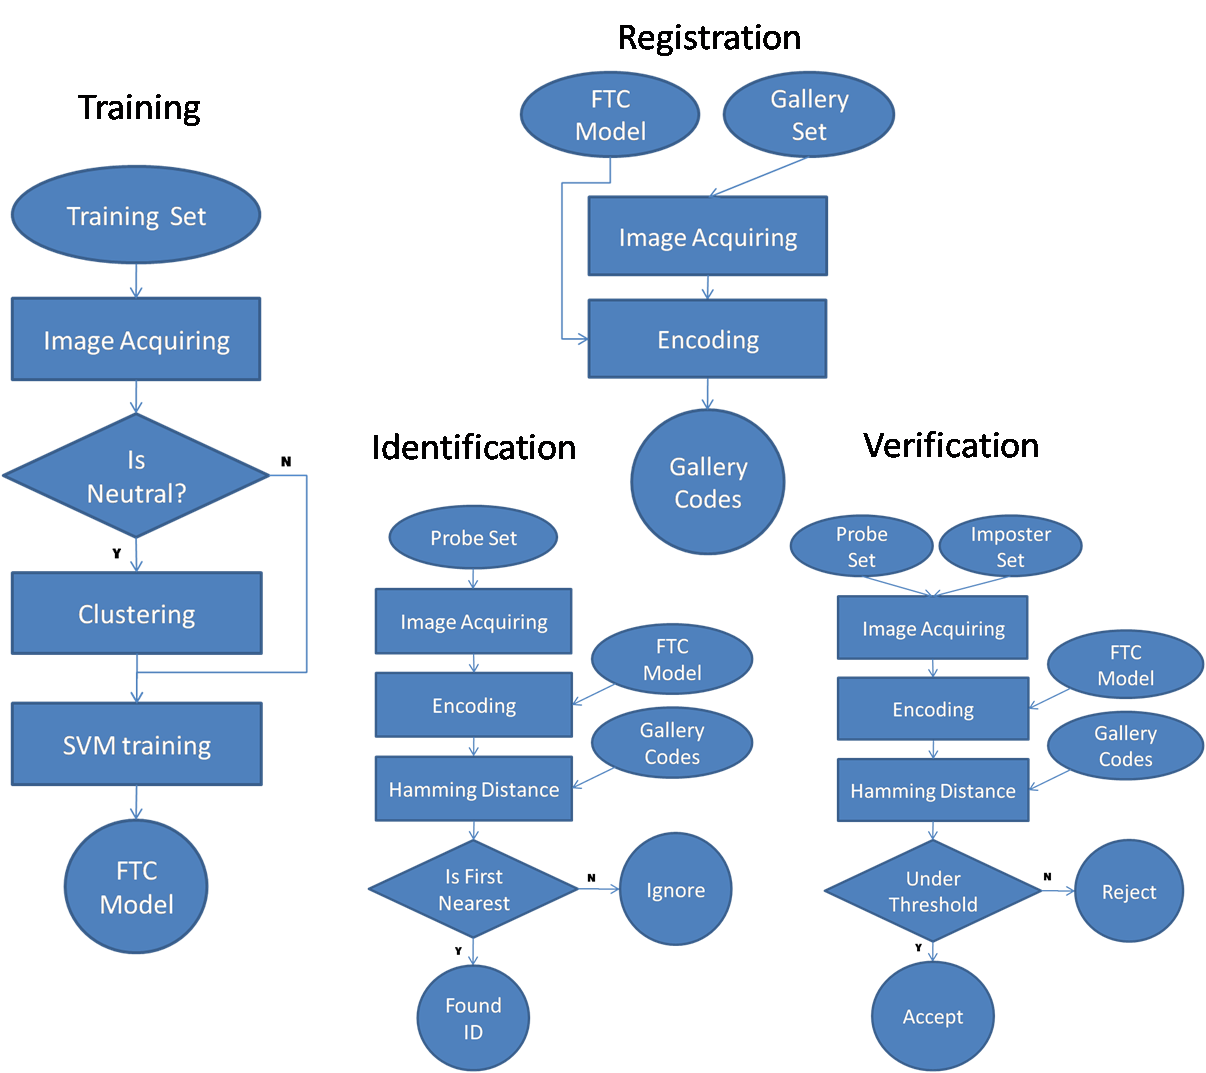
\includegraphics[width=0.8\linewidth]{fig/ftc/ftc_flow.png}
    \end{center}
    \caption{FTC working flow.}
    \label{fig:ftc_flow}
\end{figure}


We illustrate the work flow as Figure~\ref{fig:ftc_flow}. The Objects 
are defined as follow:
\begin{itemize}
    \item Training Set: Containing neutral and non-neutral images; 
    \item Gallery Set: Containing registration images;
    \item Probe Set: Testing images whose ids are in gallery set;
    \item Imposter Set: Testing images whose ids are not in gallery set;
    \item FTC Model: Containing SVM and clustering models;
\end{itemize}

Then the actions are defined as follow:
\begin{itemize}
    \item Image Acquiring: Reading images and scaling with bilinear filters, 
            and then normalizing with XmeanYstd or Adaptive Histeq;
    \item Clustering:Using PCA and LDA for dimension reduction first, 
            and then Clustering training ids for each defined patch. 
            If the patches has not defined yet, we do clustering for all possible
            patches, and then find the best ``discriminated'' patches;
    \item SVM training: For each patch, using all training images as data and clusters
            as label to train with SVM;
    \item Encoding: For each patch, applying dimension reduction,
            and then predict the cluster the patch belongs to by SVM.
    \item Hamming D: Finding bit difference between two codes as the distance.
\end{itemize}
We discuss different methods and parameters to approach the better performance.

\subsubsection{Clustering Method}
Four clustering methods are considered, {\it FJ algorithm (FJ)}, 
{\it Generalized EM (GEM)}, {\it using all ExtId as single cluster (HIE)} and
{\it Hierarchical Clustering with ``WARD'' linkage method (WARD)}.
In $k=6$ in LDA, the result plot in Figure~\ref{fig:ftc_clustering}.
We can see the best method is take the unique id in all extraction set as a
cluster, which is HIE, and then Hierarchical Clustering; The worst method is
FJ, probability the reason is the size of extraction set not big enough, so
the number of cluster is lower than GEM (average 20 clusters), HIE
(average 217 clusters).

\begin{figure}[t]
    \begin{center}
        %\fbox{\rule{0pt}{2in} \rule{0.9\linewidth}{0pt}}
        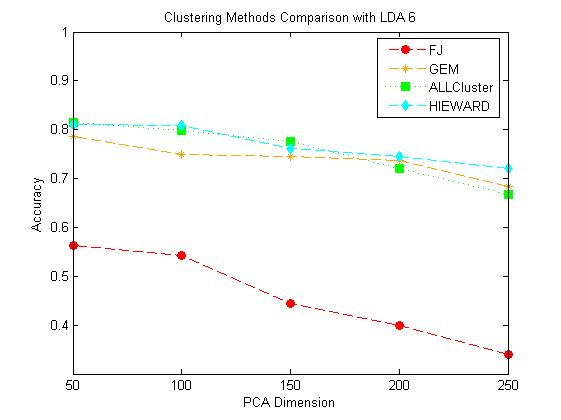
\includegraphics[width=0.8\linewidth]{fig/ftc/ftc_clustering.png}
    \end{center}
    \caption{Accuracy of FTC in different clustering methods.}
    \label{fig:ftc_clustering}
\end{figure}


\subsubsection{Different Probe Sets}
Four different faces data set are given, we plot in 
Figure~\ref{fig:ftc_sets} to see the accuracy. The pose set
in FTC and other algorithms almost have the lowest accuracy,
the expression set is not so good either. How to increase
performance in these kind of data sets may be our future works.

\begin{figure}[t]
    \begin{center}
        %\fbox{\rule{0pt}{2in} \rule{0.9\linewidth}{0pt}}
        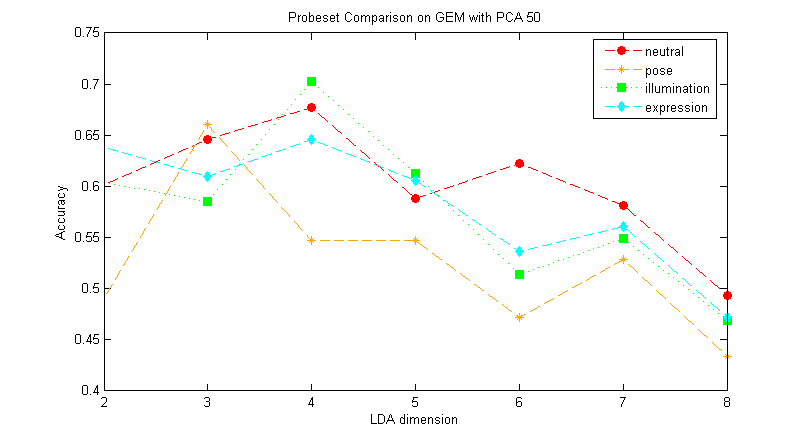
\includegraphics[width=0.8\linewidth]{fig/ftc/ftc_sets.png}
    \end{center}
    \caption{Accuracy of FTC in different probe sets.}
    \label{fig:ftc_sets}
\end{figure}


\subsubsection{PCA and LDA Dimensionality}
Different PCA and LDA dimensionalities are sensitivity in their own face 
recognition cases. Here, we discuss the influence on FTC. We show the
plot in Figure~\ref{fig:ftc_gem} and Figure~\ref{fig:ftc_hie}. As we
can see in the figures, for PCA, low dimensionality for HIE and GEM
are better. We have same observation in Fisherfaces. The reason here may
be FTC using local patches information, when the dimensionality comes bigger,
more basis with bad variance distribution would be added.
For LDA, too big dimensionality is useless in GEM, the reason may be the
number of cluster didn't increase while dimensionality increasing at the end.
However, consider about HIE, because the number of cluster is fixed,
and the scale of dimensionality of LDA is acceptable, accuracy will increase
with $k$.

\begin{figure}[t]
    \begin{center}
        %\fbox{\rule{0pt}{2in} \rule{0.9\linewidth}{0pt}}
        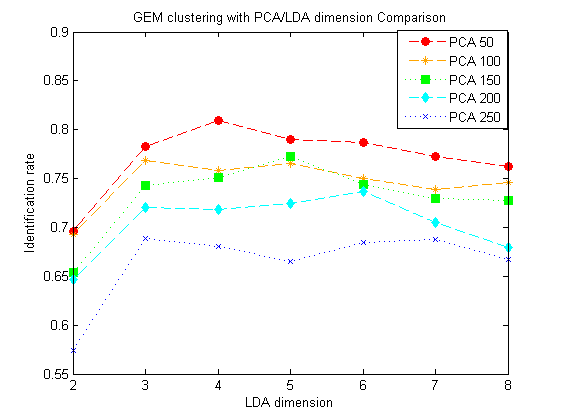
\includegraphics[width=0.8\linewidth]{fig/ftc/ftc_gem.png}
    \end{center}
    \caption{Accuracy of FTC in different PCA/LDA in GEM methods.}
    \label{fig:ftc_gem}
\end{figure}

\begin{figure}[t]
    \begin{center}
        %\fbox{\rule{0pt}{2in} \rule{0.9\linewidth}{0pt}}
        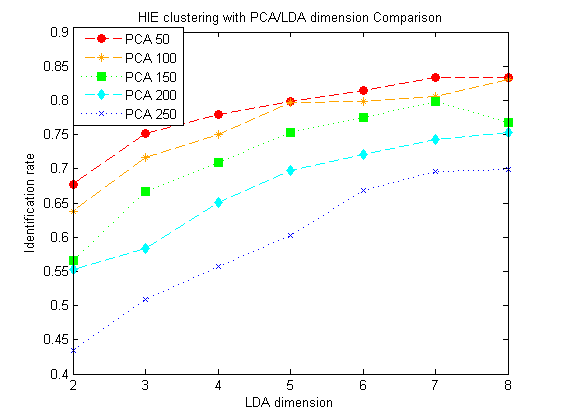
\includegraphics[width=0.8\linewidth]{fig/ftc/ftc_hie.png}
    \end{center}
    \caption{Accuracy of FTC in different PCA/LDA in HIE methods.}
    \label{fig:ftc_hie}
\end{figure}


\subsubsection{Parameters of SVM}
The library LIBSVM~\cite{CC01a} is used. For an off line training process,
we use {\it rbf kernel} for training. We have also implemented the function in
``grid.py'' and ``svm-scale.c'' for our Matlab code to approach better
tuning results. After all parameters have been set, we run a 
5-folds-cross-validation for the parameter tuning, and this step is the time bottle
neck in FTC training.

\subsubsection{Illumination Normalization}
In the illumination probe set, pixel value may have huge inconsistence with
the extraction set. We compare the recognition results of different
normalization methods: {\it 127-mean, 5-std}, {\it 127-mean, 10-std}
, above two so call {\it XmeanYstd}, and
{\it adaptive histogram equalization}, {\it no normalization}.
The result plot in Figure~\ref{fig:ftc_normalization}.
We can roughly say XmeanYstd like method is better than adaptive histogram
equalization. But the fact is there are lots of parameters can be tuned in
histogram equalization, XmeanYstd just more convenience to achieve the
better results.

\subsubsection{Image and Patch Scaling}
Image size not only influence the accuracy but also the efficiency of system.
We discuss the impact of different image and patch size using in our system.
The result plot in Figure~\ref{fig:ftc_size}. We can see different impact
in different data set. Scaling down is better for neutral face data set,
but get the worst result in illumination data set. We believe that scaling
the image and patch has strong data set dependency.

\begin{figure}[t]
    \begin{center}
        %\fbox{\rule{0pt}{2in} \rule{0.9\linewidth}{0pt}}
        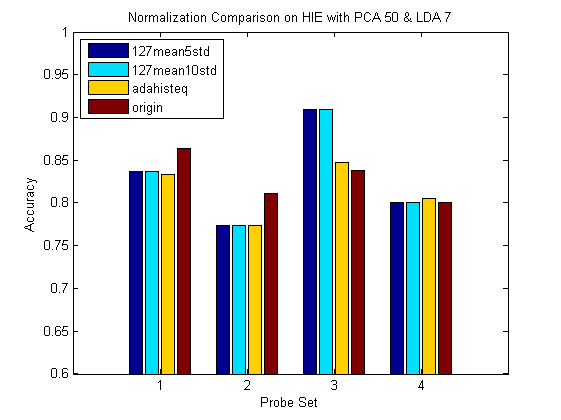
\includegraphics[width=0.8\linewidth]{fig/ftc/ftc_normalization.png}
    \end{center}
    \caption{Accuracy of FTC in different normalization methods. (neutral, pose, illumination, Expression)}
    \label{fig:ftc_normalization}
\end{figure}

\begin{figure}[t]
    \begin{center}
        %\fbox{\rule{0pt}{2in} \rule{0.9\linewidth}{0pt}}
        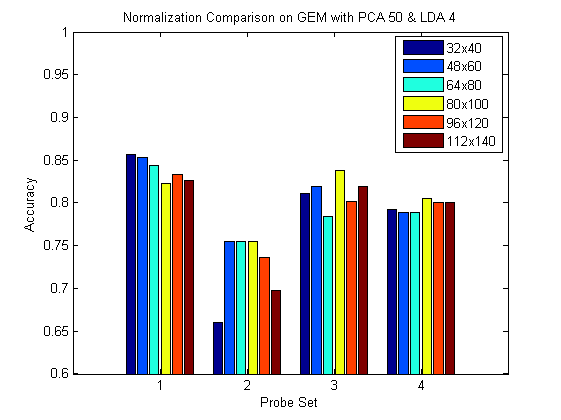
\includegraphics[width=0.8\linewidth]{fig/ftc/ftc_size.png}
    \end{center}
    \caption{Accuracy of FTC in different image and patch size. (neutral, pose, illumination, Expression)}
    \label{fig:ftc_size}
\end{figure}

\subsubsection{The Number of Patch Used}
Consider all 63 patches we are given, there is a possible that the patch
redundancy effected the discrimination influence the accuracy. We illustrate the 
result in Figure~\ref{fig:ftc_npatch}. The accuracy is not increase monotonically,
just like we mention, however, the trend is proportion to number of patch size.

\begin{figure}[t]
    \begin{center}
        %\fbox{\rule{0pt}{2in} \rule{0.9\linewidth}{0pt}}
        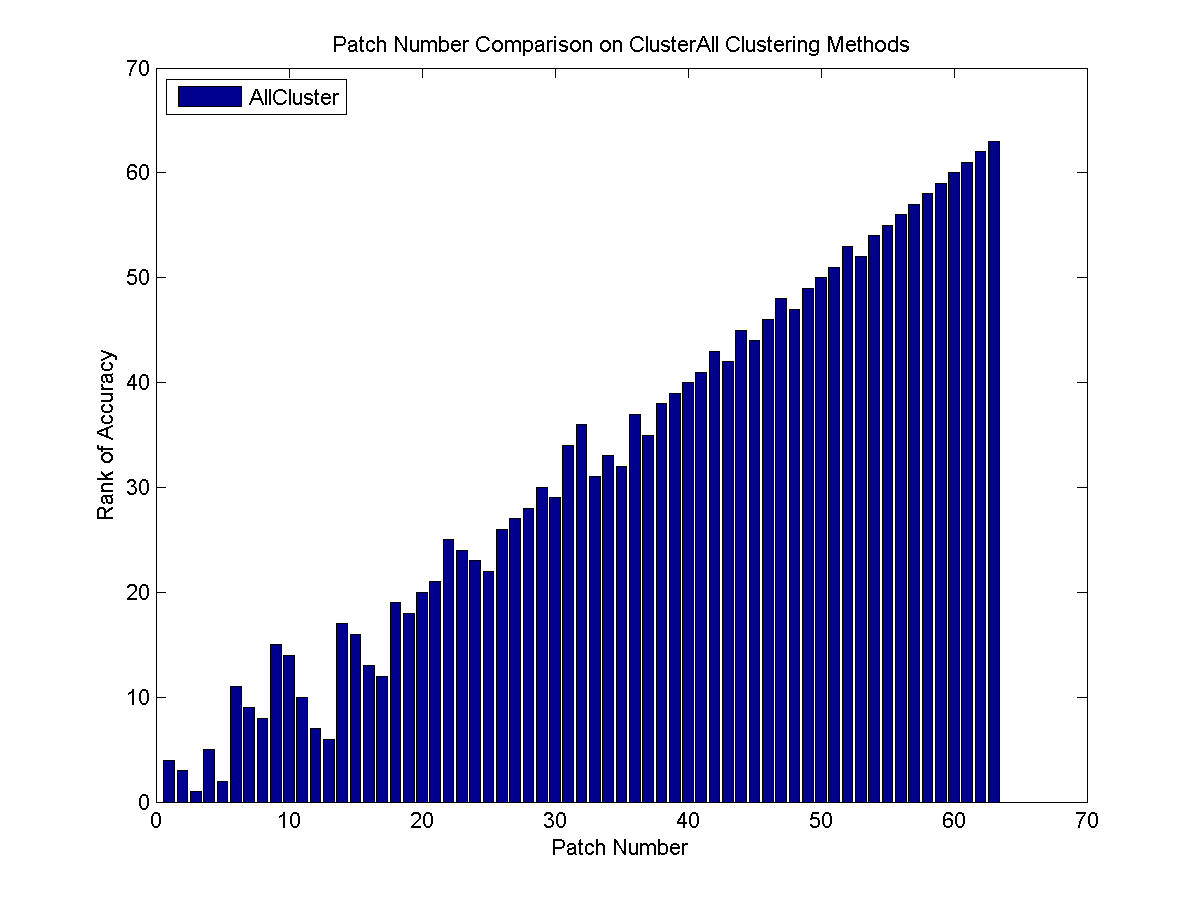
\includegraphics[width=0.8\linewidth]{fig/ftc/ftc_npatch.png}
    \end{center}
    \caption{Ranking of accuracy of FTC in different number of patch used.}
    \label{fig:ftc_npatch}
\end{figure}


\subsection{FTC Patch Finding}
In addition to the $63$ best patches which are given, the algorithm of Facial Trait has
been implemented for finding our own $256$ best patches. The result shows in
Figure~\ref{fig:ftc_ownpatch}. Surprisingly, besides the illumination set,
our patches has better accuracy. We bring up some possible answers.
\begin{enumerate}
    \item Our parameters are different.
    \item The training set of 1815 images is relative smaller than the paper purpose.
    \item Four times patches we used in the experiment.
\end{enumerate}
The ranking of accuracy of different patch size is plotted in 
Figure~\ref{fig:ftc_rank}. The accuracy of using $256$ patches will gain
$1$ to $3\%$. The patches we found show in Fiugre~\ref{fig:ftc_256}.

\begin{figure}[t]
    \begin{center}
        %\fbox{\rule{0pt}{2in} \rule{0.9\linewidth}{0pt}}
        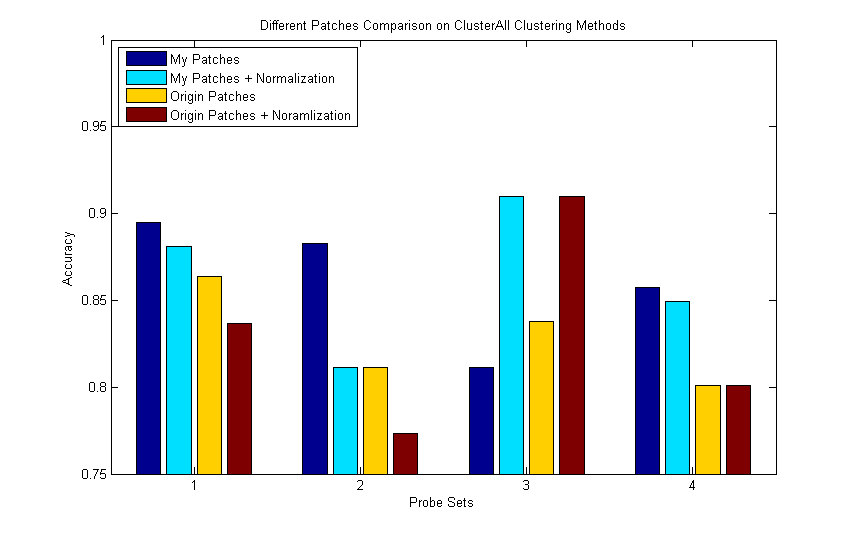
\includegraphics[width=0.8\linewidth]{fig/ftc/ftc_ownpatch.png}
    \end{center}
    \caption{Accuracy of FTC in different patch sets. (neutral, pose, illumination, Expression)}
    \label{fig:ftc_ownpatch}
\end{figure}

\begin{figure}[t]
    \begin{center}
        %\fbox{\rule{0pt}{2in} \rule{0.9\linewidth}{0pt}}
        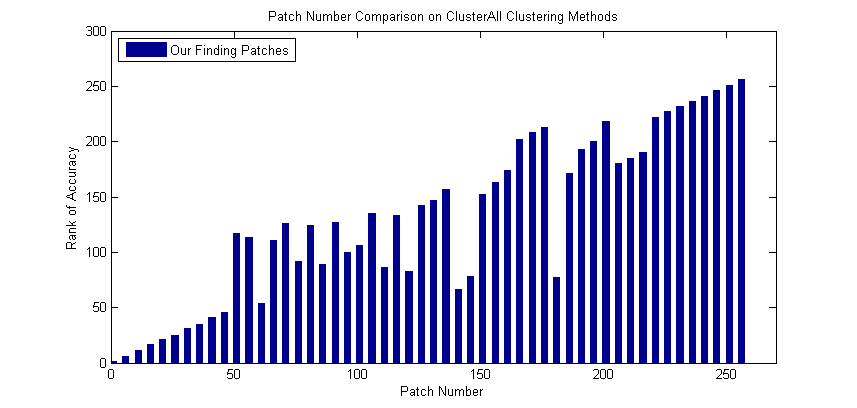
\includegraphics[width=0.8\linewidth]{fig/ftc/ftc_rank.png}
    \end{center}
    \caption{Ranking of accuracy of FTC in our patches.}
    \label{fig:ftc_rank}
\end{figure}

\begin{figure}[t]
    \begin{center}
        %\fbox{\rule{0pt}{2in} \rule{0.9\linewidth}{0pt}}
        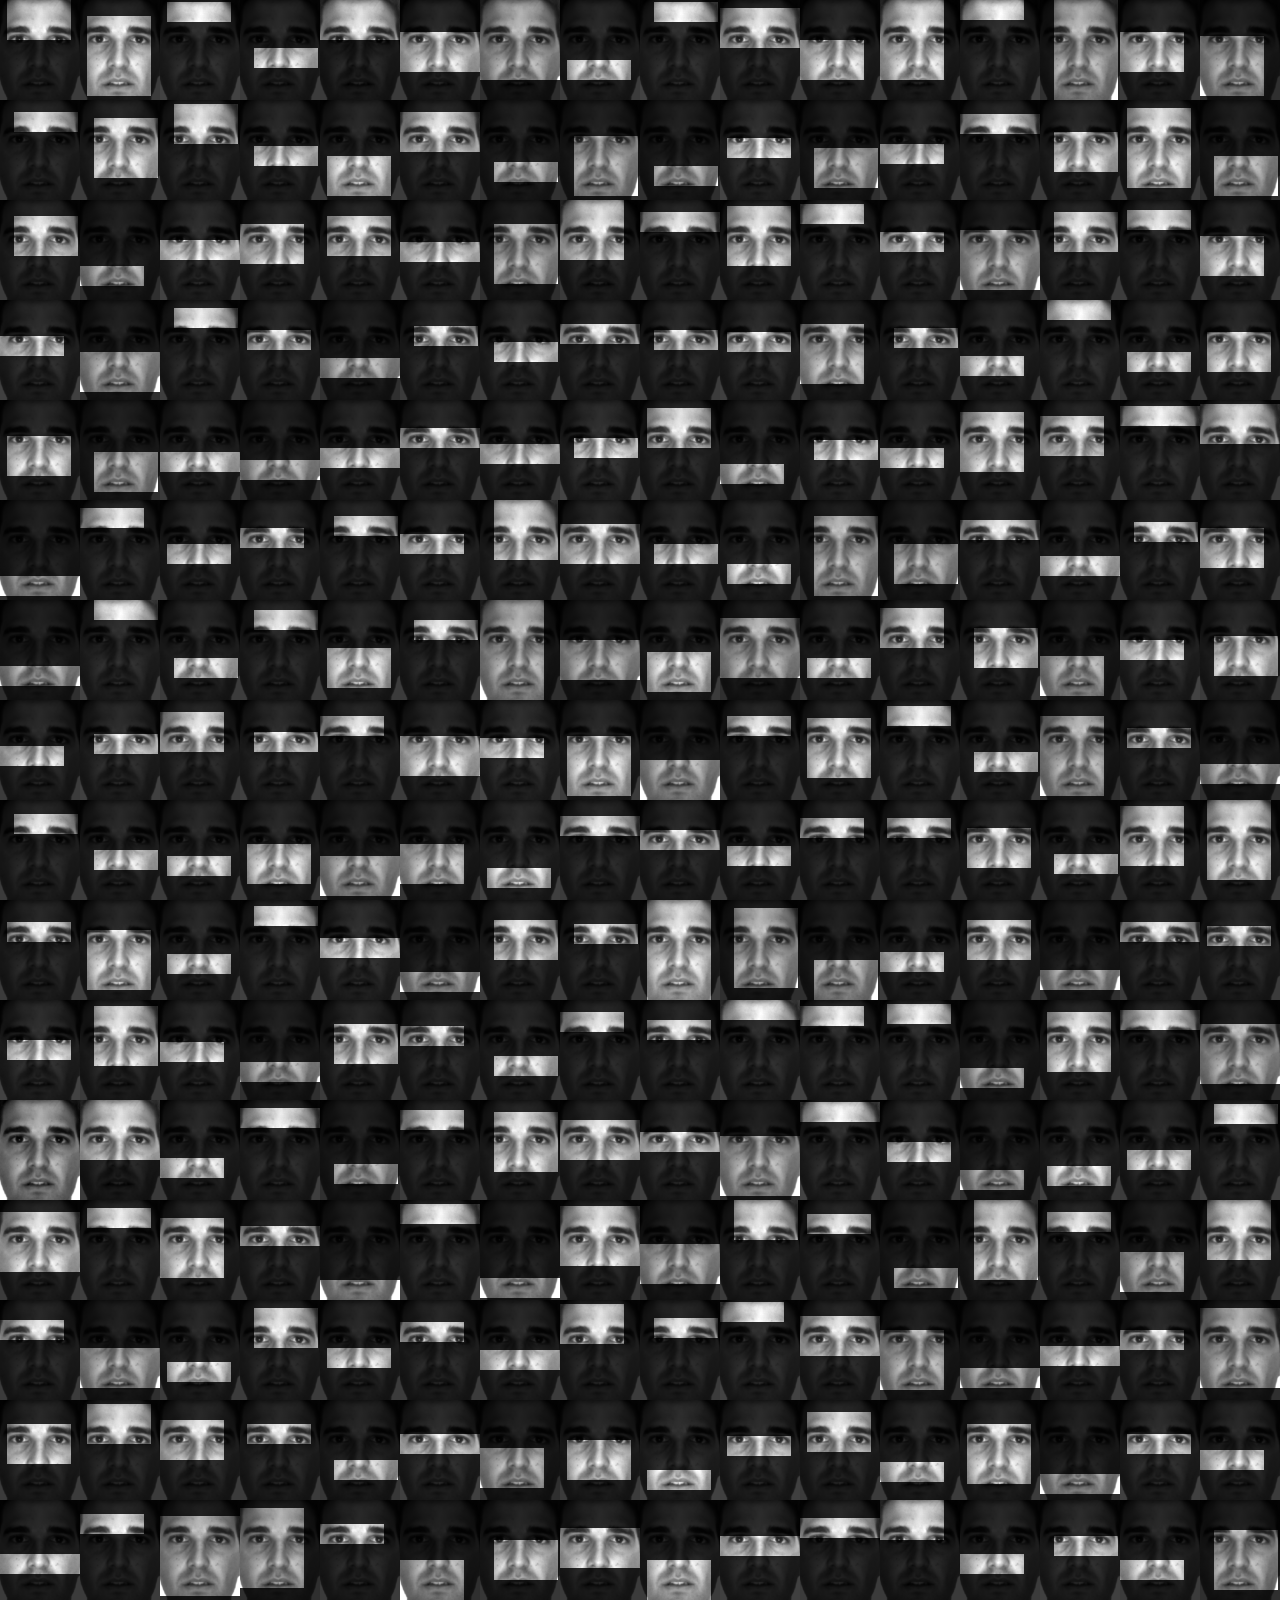
\includegraphics[width=0.8\linewidth]{fig/ftc/ftc_256.png}
    \end{center}
    \caption{Our patches fined by Facial Trait Algorithm.}
    \label{fig:ftc_256}
\end{figure}



\subsection{Face Verification Using FTC}
In face verification process, we sum up $P$ faces in all probe set and
$I$ faces in imposter set as testing images, to test all $G$ 
possible register id. Therefore, we have $N*G$ test data, $P's$ truth and
$N*G-P's$ false. So different threshold can refer to different ROC curve.
Refer Figure~\ref{fig:ftc_roc_com}, we get better ROC curve by 
using our own patches with HIE. The figure also points
that normalization with GEM using in face verification can improve the ROC curve.
Consider both Figure above, we find out the neutral faces data set has better
verification performance, and pose faces data set has the worst one. 
For clustering methods, HIE is better than GEM in our experiment.

\begin{figure*}[t]
    \begin{center}
        %\fbox{\rule{0pt}{2in} \rule{0.9\linewidth}{0pt}}
        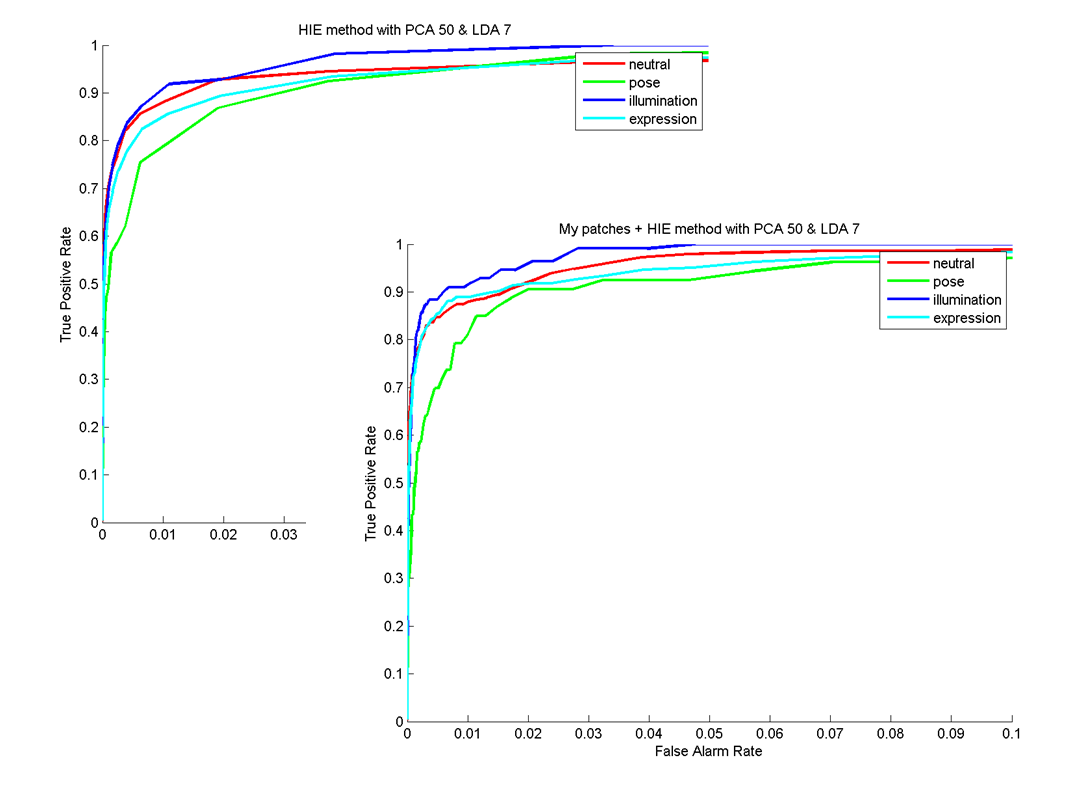
\includegraphics[width=0.4\linewidth]{fig/ftc/ftc_roc_com1.png}
        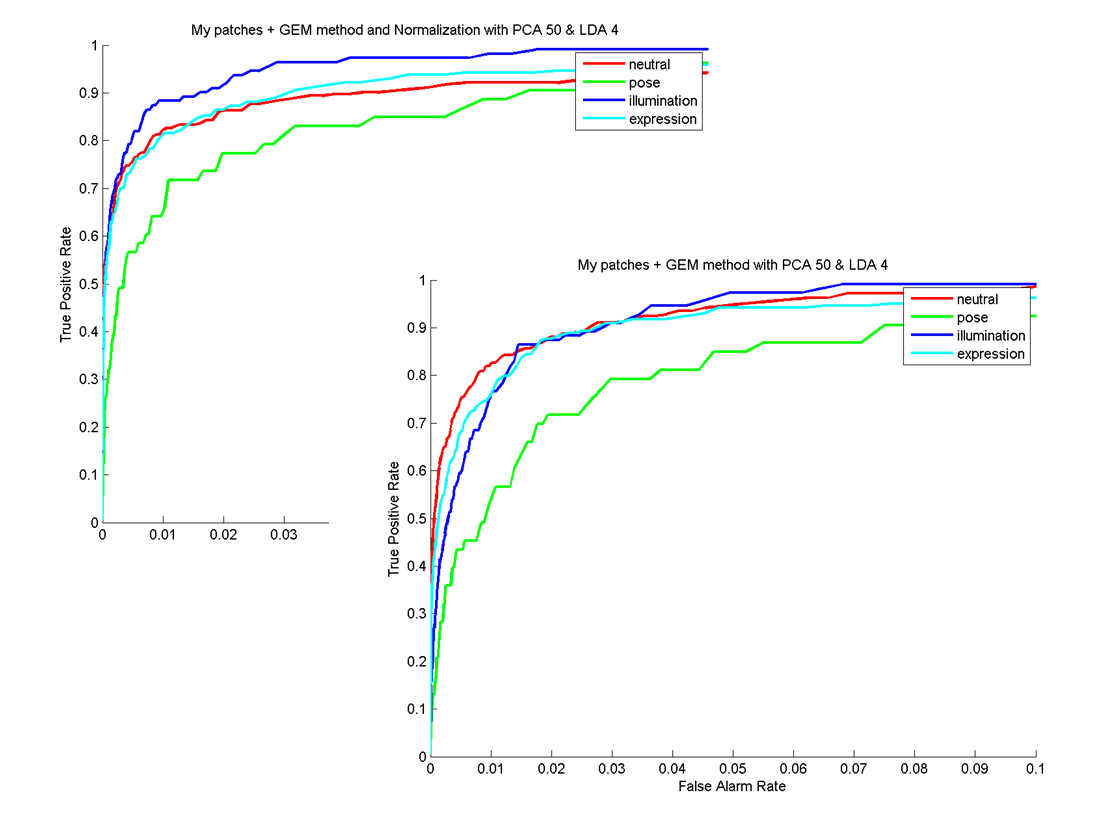
\includegraphics[width=0.4\linewidth]{fig/ftc/ftc_roc_com2.png}
    \end{center}
    \caption{ROC curve experiment.}
    \label{fig:ftc_roc_com}
\end{figure*}


\subsection{System Performance in FTC}
The development environment is on $64$ bits Linux workstation, coding in Matlab.
The FTC performance in different algorithms are average between $0.07$ and $1.05$
seconds per image. The result shows in Figure~\ref{fig:ftc_time}.
Clearly, FTC identification rate is proportion to the number of patches and
the number of clusters. How to trade off performance and identification rate
is an important issue.

\begin{figure}[t]
    \begin{center}
        %\fbox{\rule{0pt}{2in} \rule{0.9\linewidth}{0pt}}
        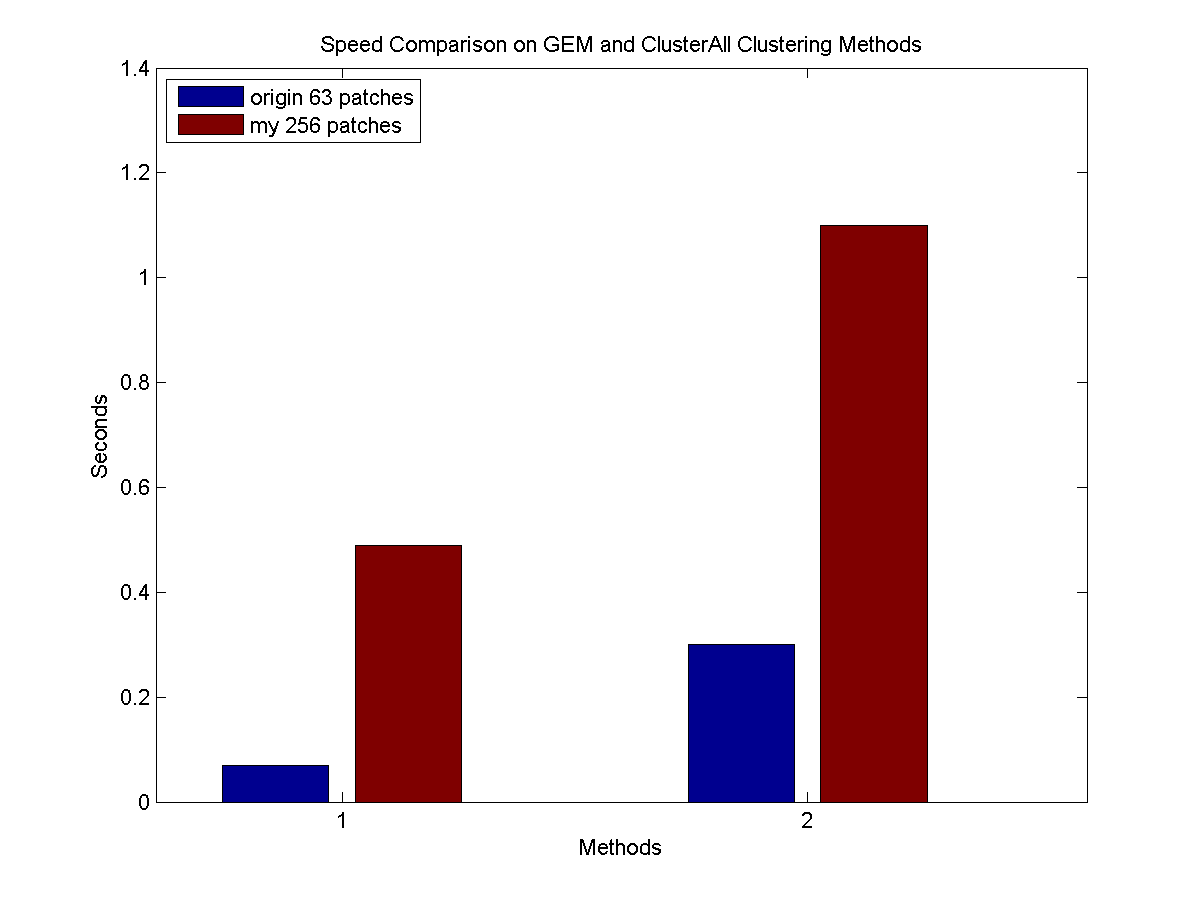
\includegraphics[width=0.8\linewidth]{fig/ftc/ftc_time.png}
    \end{center}
    \caption{System performance of FTC.}
    \label{fig:ftc_time}
\end{figure}



%-------------------------------------------------------------------------
%-------------------------------------------------------------------------
%-------------------------------------------------------------------------

\subsection{Ensemble Voting Algorithm}
Ensemble learning is widely used in lots of applications. Here we try to 
gather LDA, LBP and FTC to vote the best decision. The Ensemble Voting Algorithm
(EVA) is described
as follow:
\begin{enumerate}
    \item LDA, LBP and FTC have their own decision. Only FTC can judge
          the visitor is imposter or guest.
    \item If three algorithms decide to output the same face id, there is no problem.
    \item Else if two of algorithms have the same face id, if one of the algorithm
          is FTC, than truth the idea.
    \item However, if LDA and LBP have the dame face id, then must ask FTC first.
            If the threshold of FTC is not higher enough. Then truth other two's
            decision.
\end{enumerate}
The accuracy of EVA has reported in Section 3.. Under this criteria, EVA is
hard to plot the ROC curve, because the distance matrix is can not be define.

%-------------------------------------------------------------------------

\section{Performance Report}
In this section, we report the ROC curve and the accuracy rate we achieve
in different methods. The accuracy of four methods testing without imposter
are showed in Table~\ref{tab:acc}. The accuracy of EVA testing with imposter
is showed in Table~\ref{tab:eva}. The ROC curve of four methods are reported
in Figure~\ref{fig:roc}.

\begin{figure*}[t]
    \begin{center}
        %\fbox{\rule{0pt}{2in} \rule{0.9\linewidth}{0pt}}
        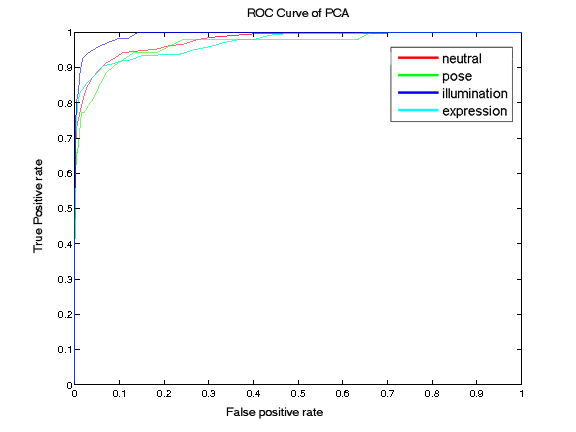
\includegraphics[width=0.4\linewidth]{fig/pca/pca_roc.png}
        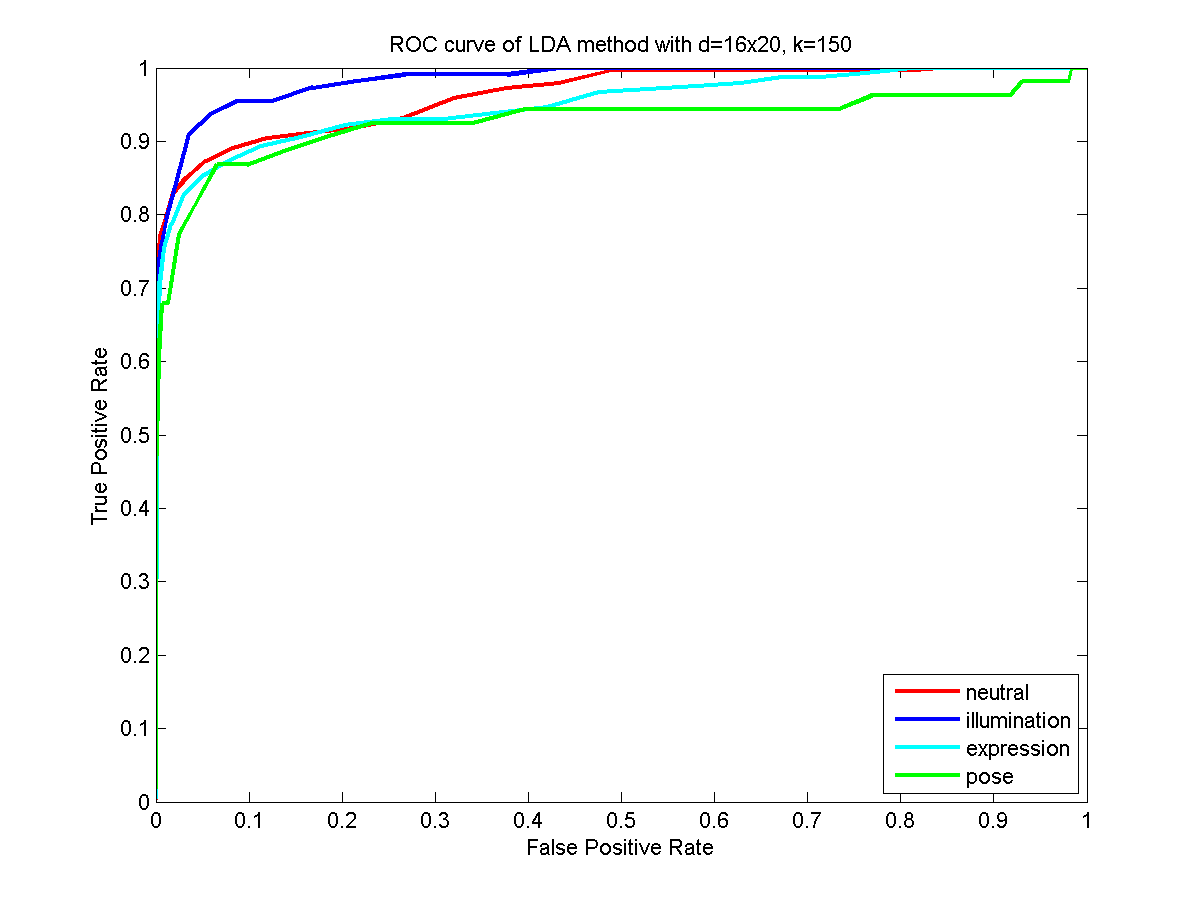
\includegraphics[width=0.4\linewidth]{fig/lda/lda_roc.png}
        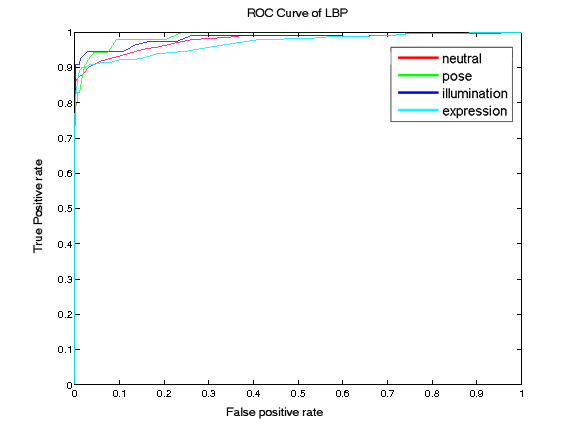
\includegraphics[width=0.4\linewidth]{fig/lbp/lbp_roc.png}
        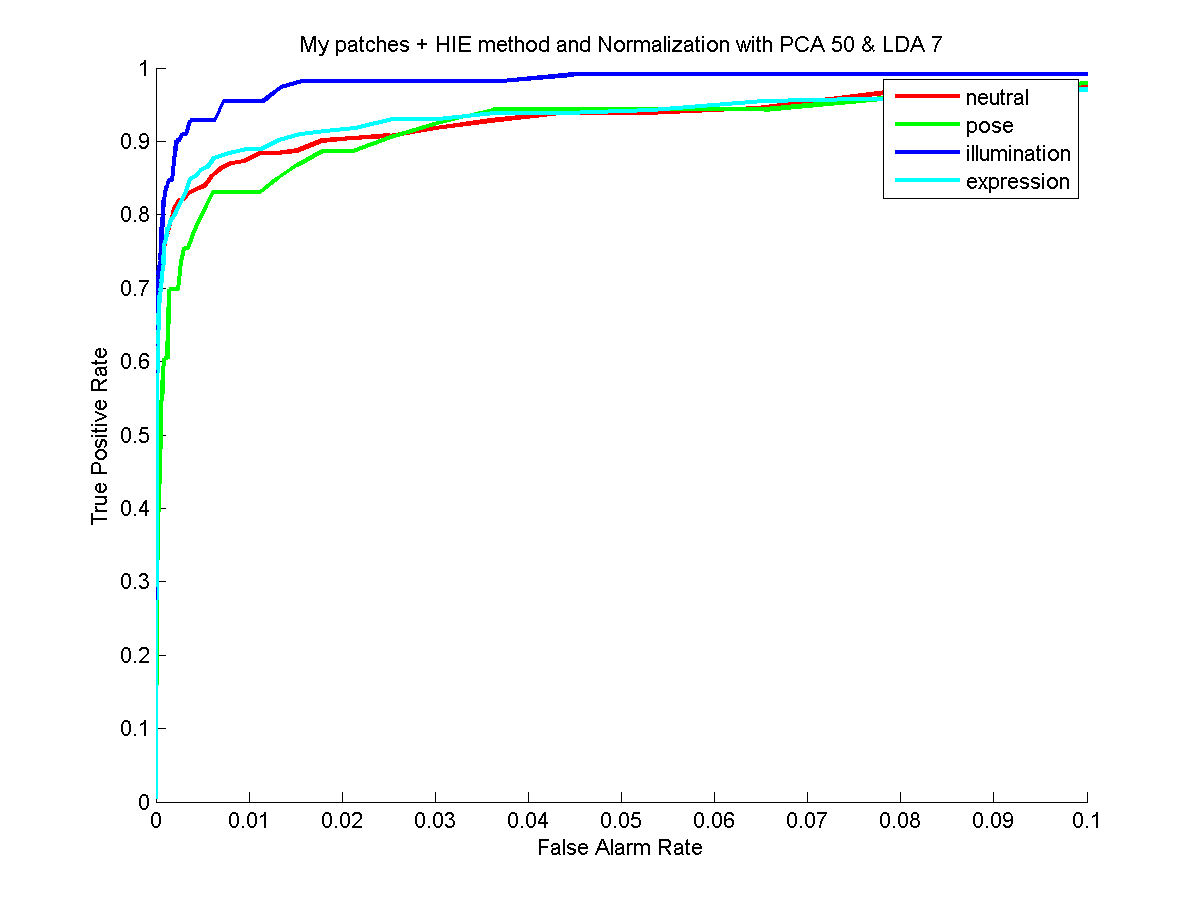
\includegraphics[width=0.4\linewidth]{fig/ftc/ftc_roc.png}
    \end{center}
    \caption{ROC curve}
    \label{fig:roc}
\end{figure*}


\begin{table}
    \begin{center}
        \begin{tabular}{|l|c|c|c|c|}
            \hline
            Methods & Neutral & Illumination & Expression & Pose\\
            \hline\hline
            PCA & 0.8027 & 0.8108 & 0.8455 & 0.7736 \\
            LDA & 0.9150 & 0.9189 & 0.8902 & 0.8302 \\
            LBP & {\bf 0.9422} & {\bf 0.9730} & {\bf 0.9106} & {\bf 0.9245}\\
            FTC & 0.8810 & 0.9099 & 0.8496 & 0.8113 \\
            \hline
        \end{tabular}
    \end{center}
    \caption{Accuracy of four methods tested without imposter.}
    \label{tab:acc}
\end{table}

\begin{table}
    \begin{center}
        \begin{tabular}{|l|c|c|c|c|}
            \hline
            Methods & Neutral & Illumination & Expression & Pose\\
            \hline\hline
            EVA & 0.8844 & 0.8739 & 0.8455 & 0.7925 \\
            \hline
        \end{tabular}
    \end{center}
    \caption{Accuracy of EVA with imposter.}
    \label{tab:eva}
\end{table}


%-------------------------------------------------------------------------

\section{Conclusions and Future Works}
About the experiment results. We find out PCA and LDA have preliminary successes
in face recognition problem. After that, LBP achieves the highest accuracy
in different probe sets in our experiment. 
In the end, FTC provides the best ROC curve for the whole system.
EVA also achieve good  performance in the random testing, the thing is we
try different way to approach the goal, and find out ensemble learning scheme
is also work in face recognition problem.

We implement five different methods and compare each method via report
the system accuracy in types of faces data sets, and their ROC curves.
The system may not so perfect, therefore, we point several problems and
discussions for future work.

One problem is for all algorithms, no one is good at dealing with the pose faces set,
a new kind of normalization scheme should be considered. Second, shape like features
is powerful when used in face recognition problem, we may try to develop a new kind
of feature descriptor for this. In the end, ensemble learning scheme have lots of
division, this is also a good way for researching.

%-------------------------------------------------------------------------
%------------------------------------------------------------------------

{\small
\bibliographystyle{ieee}
\bibliography{egbib}
}

%\newpage
%\rule{0pt}{1pt}\newpage
%\rule{0pt}{1pt}\newpage
%\rule{0pt}{1pt}\newpage
%\rule{0pt}{1pt}\newpage
%\rule{0pt}{1pt}\newpage
%\rule{0pt}{1pt}\newpage
%\rule{0pt}{1pt}\newpage
%\rule{0pt}{1pt}\newpage

\end{document}
